\documentclass{article}[11pt]
\usepackage[left=1.0in, right=1.0in, top=1.0in, bottom=1.0in,nohead]{geometry}              		
\geometry{letterpaper}

\usepackage{graphicx, grffile}														
\usepackage{amssymb, amsmath, amsfonts}
\usepackage{setspace}
\usepackage{titlesec}
\usepackage[usenames, dvipsnames]{color}
\usepackage{soul}
\usepackage{float, multirow, tabulary}
\usepackage{subcaption}

\newcommand{\bp}[1] {\left( #1 \right)}
\newcommand{\bb}[1] {\left[ #1 \right]}
\newcommand{\ba}[1]{\left| #1 \right|}
\newcommand{\infint}{\int_{-\infty}^\infty}

\titleformat{\section}{\Large\bfseries}{\thesection}{0.5em}{}
  
\titleformat{\subsection}{\normalfont\normalsize\bfseries}{\thesubsection}{0.5em}{}

\titleformat{\subsubsection}{\normalfont\normalsize\bfseries\itshape}{\thesubsubsection}{0.5em}{}  
  
\titlespacing{\section}{0pt}{0pt}{2pt}

%\newcommand{\kbcom}[1]{
%\textcolor{blue}{\textbf{\textit{\ul{#1}}}}}
%
%\newcommand{\blcom}[1]{
%\textcolor{red}{\textbf{\textit{\ul{#1}}}}}         
%
%\newcommand{\llcom}[1]{
%\textcolor{Orange}{\textbf{\textit{\ul{#1}}}}}
%
%\newcommand{\tlcom}[1]{
%\textcolor{LimeGreen}{\textbf{\textit{\ul{#1}}}}} 

\newcommand{\Matlab}{\textsc{Matlab}}

\title{Final Report on Analyzing Time-Frequency Methods and Unsupervised Clustering Algorithms for Footstep Classification}
\author{Group Members: Kaitlyn Beaudet, Brett Larsen, Lydia Letham, Tianran Liu}
\date{}


%%%%%%%%%%%%%%%%%%%%%%%%%%%%%%%%%%%%%%%%%%%%%%%%%%%%%%
%								REQUIREMENTS									%
% Project Title																		%
% Name(s) of team member(s)															%
% 17 <= #pg <= 20																	%
% Additional Pages allowed for Matlab code or equation derivations								%
% Abstract of 100-150 words															%
%	- Provide concise statement of the initial problem and related background						%
%	- Describe methodology and key findings												%
%	- Describe major conclusions														%
% References must be less than one page												%
% Introduction/Motivation* why the problem is important, organization for the rest of the report., main refs	%
% Background 																		%
% Problem Formulations 																%
% Theoretical Solutions																% 
% Simulations/Results																%
% Work Managament*- must write our own subsections, which < 1pg, tasks including paper division		%
% Conclusions* - main results and deductions												%
% Acknowledgements																%
%%%%%%%%%%%%%%%%%%%%%%%%%%%%%%%%%%%%%%%%%%%%%%%%%%%%%%

\begin{document}
\maketitle
\doublespace

%\vspace{-30pt}

\begin{abstract}
The purpose of this project was to determine if vibration signals could be detected and classified for purposes such as security along borders or other sensitive boundaries. To this end, the goal was to see if footsteps could be correctly detected and classified within different groups. Many different analysis techniques were to be attempted, and then feature extraction and classification was performed on the outputs. It was found that RID, WD, and MPD were successful in distinguishing an adult from a child, an adult running from an adult walking, a child running from a child walking, and two adults versus three adults.  Future work will include the investigation of other feature extraction methods and unsupervised clustering.
\end{abstract}

\section{Introduction}
\label{sec:intro}
The problem of detecting and classifying vibration signals produced by footsteps has applications in a variety of areas, especially in those associated with national security. These applications include that of alerting authorities to activity along a  border or around a nuclear power plant or even around an entire base in hostile territory. To this end, the goal of this project is to accurately detect and classify different classes of footsteps without false positives caused by friendly forces or natural elements such as animal traffic or blowing plant life (e.g. tumbleweeds). In order to observe the feasibility of time-frequency techniques in such classification purposes, an attempt will be made to detect and classify different movement patterns produced by different groups of adults, children and animals, both walking and running. This data will be analyzed using techniques such as the Spectrogram, Ambiguity Function, Wigner Distribution, Reduced Interference Distribution, as well as matching pursuit decomposition. Features will be extracted from the outputs of these methods and used to classify the signals.

In Section \ref{sec:background} the background and motivation of the project is discussed. The methods of data acquisition by the team are discussed in Section \ref{sec:data}, and Section \ref{sec:methods} delineates how the data was processed to complete the main goal of footstep classification.  In Section \ref{sec:results}, the results gained from \Matlab \ are provided and discussed. Section \ref{sec:work} describes the work that each team member accomplished through the course of this project.

%%%%%%%%%%%%%%%%%%%%%%%%%%%%%%%%%%%%%%%%%%%%%%%%%%%%%%
%\vspace{-10pt}
\section{Background}
\label{sec:background}
Footstep detection and classification have received a great deal of attention in recent years because of the vital role this area plays in remote operations, such as perimeter protection, curtailing illegal border crossings, and alerting authorities to activity in critical areas \cite{Mehmood2012}. Thus, detecting and classifying vibration signals produced by footsteps has become a very active research topic. In 2001, George Succi, Daniel Clapp and Robert Gampert proposed the idea to use seismic amplitude distributions, such as kurtosis, to identify a footstep \cite{Succi2001}. Later in 2003, Houston and McGaffigan proposed a novel footstep detection algorithm using cadence features instead of the conventional approach of detecting transients corresponding to individual footfalls. They examined the use of spectrum analysis on envelope-detected seismic signals and obtained good results \cite{Houston2003}. Then, in 2006, Bland discussed the use of autoregressive (AR) coefficients in designing a footstep detection scheme from acoustic and seismic sensors \cite{Bland2006}. Next, in 2007,  Damarla considered using a multi-modal multi-sensor fusion algorithm for the detection of personnel. In particular, he employed unattended ground sensors consisting of acoustic, seismic, and passive infrared (PIR) sensors along with a video camera \cite{Damarla2007}. In 2009, Subramanian considered employing empirical mode decomposition (EMD)-based signal processing scheme for the detection of footsteps \cite{Subramanian2009}.  More recently, in 2011, Thyagaraju Damarla and James Sabatier from the U.S. Army Research Laboratory presented work on developing algorithms to detect and classify people walking and jogging based on the fact that when people are moving fast, the impact of their foot on the ground is more intense and a higher Doppler signature from an ultrasonic sensor can be observed \cite{Damarla2011}. Finally in 2012, Asif Mehmood and Thyagaraju Damarla utilized seismic data and time-frequency techniques to distinguish human footsteps from horse footsteps \cite{Mehmood2012}. 


However, these experiments have certain limitations. As an expansion upon previous research that mainly focused on simple horse, person walking, person running classification, the team collected data of an adult walking, adult running, child walking, child running, dog walking and dog running and attempted to classify different categories. The team also compared different methods of feature extraction and time-frequency classification methods to determine which yields the best results.

%%%%%%%%%%%%%%%%%%%%%%%%%%%%%%%%%%%%%%%%%%%%%%%%%%%%%%
%\vspace{-10pt}
\section{Data Acquisition}
\label{sec:data}
In order to determine which method would work best for the detection and classification of footsteps, the team collected real data. The data collection took place in an environment similar to that of the Southwest border, and all the data was collected at the same time. The consistency of the environment was important as it helped to reduce the effect of parameters outside the scope of our project such as the noise, terrain type, and weather. 

Eight GS-One geophone sensors were used in the geometry of a single straight line approximately eight inches apart, as illustrated below in Figure \ref{fig:Path}. The subjects would run past the sensors attempting to stay the same distance away from each one. For each trial, the subject would start from the other end of the sensors (i.e. if trial one started at sensor one, trial two would start from sensor eight). The data was collected using two NI DAQ cards connected to two computers and collected via the Data Acquisition Toolbox in \Matlab. The sensor information was saved into matrices which were exported for later use. Due to technological constraints, for some trials, data was only collected from four sensors as one of the computers connected to the DAQ cards ran out of power.

\begin{figure}[h!]
   \centering
   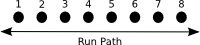
\includegraphics{Images/Path.png} 
   \caption{Experimental Setup}
   \label{fig:Path}
\end{figure}

The categories to be analyzed were that of a child alone, an adult and a child, an adult and a dog, an adult alone, two adults and three adults. For each category, data was collected for the subject(s) both running and walking. In cases where it was possible, data was gathered for additional subjects that met the requirements. Specifically, four different adults performed the individual trials, and two different adults performed the trials with the same dog. 
%%%%%%%%%%%%%%%%%%%%%%%%%%%%%%%%%%%%%%%%%%%%%%%%%%%%%%
%\vspace{-10pt}
\section{Methods}
\label{sec:methods}
To attempt classification, many different methods were used to generate the time-frequency representations (TFRs) to be classified.
\subsection{Data Preprocessing}
Before the time-frequency methods were performed on the collected data, some preprocessing was completed. This was done to make the run time for the data with the time-frequency methods discussed in \ref{sec:analysis} more manageable. First, the signal was down-sampled by two, effectively halving the length of the data vectors, while still retaining the necessary information. After the downsampling was completed, the data was centered around the maximum and only a small region around the maximum was selected for analysis. By doing this, the team was able to further cut down the number of samples. This was accomplished by selecting only some of the values from the down-sampled matrix, taking half of the new vector samples from one side of the maximum and the other half to the other side of the maximum. Thus, each of the new vectors contained the same span of time, however, contained the most important spans for each of the data vectors. Finally, prior to the time-frequency analysis, the analytic part of the signal was taken by performing a Hilbert transform on the down-sampled, centred data vector. This reduces aliasing for methods such as the Wigner Distribution and Reduced Interference Distribution discussed in Sections \ref{sec:WD} and \ref{sec:RID} respectively.
\subsection{Analysis Techniques}
\label{sec:analysis}
\subsubsection{Matching Pursuit Decomposition}
\label{sec:MPD}
Matching pursuit decomoposition (MPD) is an iterative methods that decomposes a signal in terms of representative basis functions, which are in this case cosine-modulated Gaussions.  After constructing an entire dictionary of Gaussion signals, MPD uses the inner product the find the dictionary element that best mathces the input signal.  This dictionary signal is then subtracted out of the input and the Gaussian parameters are stored before repeating the process again.  As explained in \cite{Larsen2013}, the time-frequency representation for MPD can be expressed the following way:
\begin{equation}
\uppercase{\epsilon}_s(t,f) \equiv \sum^{N-1}_{i=0} |\kappa_{i}|^{2} WD_{g_{i}}(t,f),
\end{equation}
where $WD_g(t, f)$ is the Wigner distribution of $g(t)$, given for the Gaussian atoms by
\begin{equation}
WD_g(t, f) = 2\exp(-\alpha(t-\tau)^2) \exp\left(\frac{2\pi^2(f-\nu)^2}{\alpha}\right).
\end{equation}
and $|\kappa_{i}|^{2}$ represents the coeffiecients that determine the relative weighting of each individual Gaussian term.
Figures \ref{fig:MPDTFR1} and \ref{fig:MPDTFR2} below depict examples of the TFR formed by features extracted by the MPD from the data gathered.


\begin{figure}[H]
\centering
\begin{minipage}[b]{0.45\linewidth}
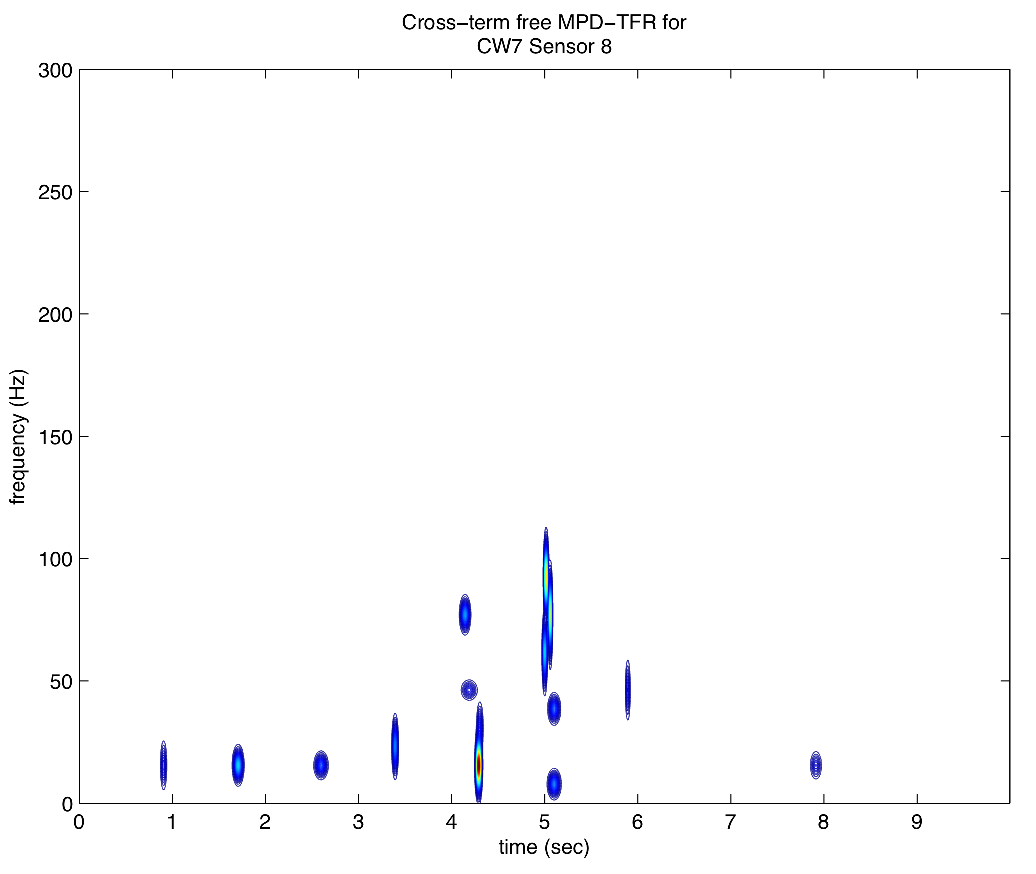
\includegraphics[scale = 0.4]{Images/MPD.pdf}
\caption{Example of an MPD TFR (Child Walking)}
\label{fig:MPDTFR1}
\end{minipage}
\hfill
\begin{minipage}[b]{0.45\linewidth}
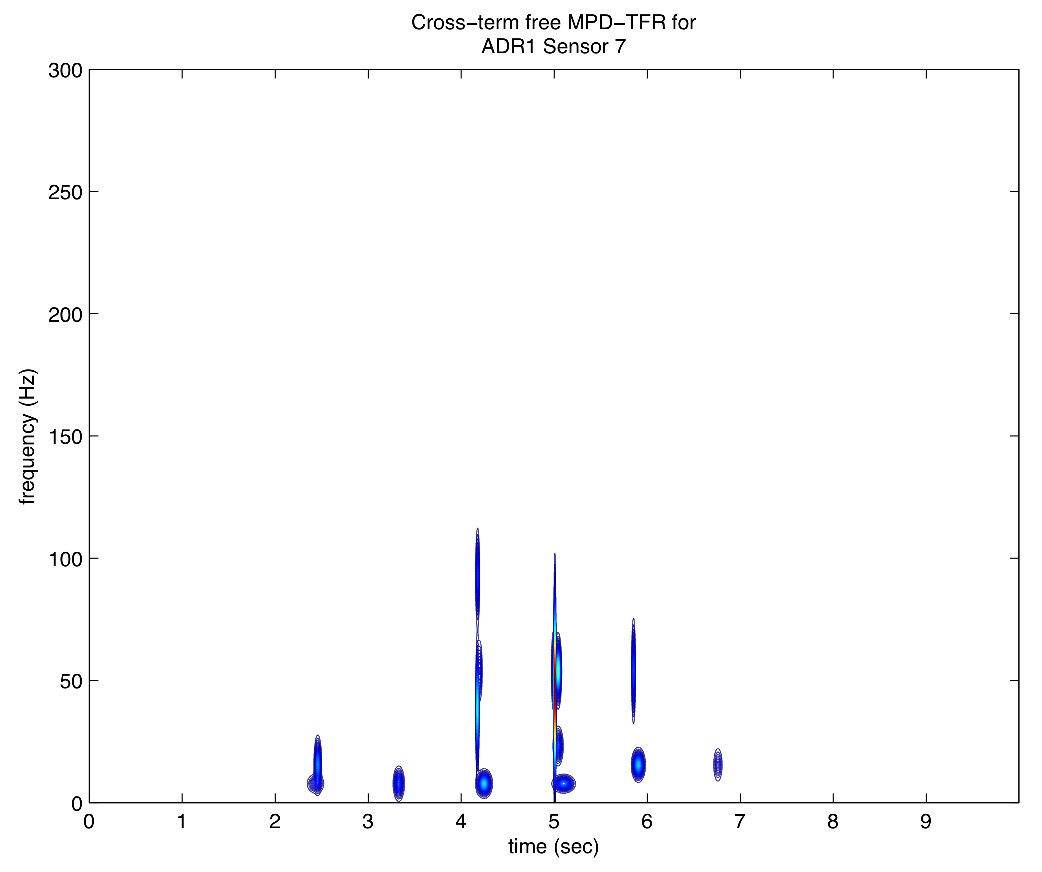
\includegraphics[scale = 0.4]{Images/MPD2.pdf}
\caption{Second Example of an MPD TFR (Adult Running)}
\label{fig:MPDTFR2}
\end{minipage}
\end{figure}

MPD was used in two different ways in the project.  First, like all other the other methods, it was first used to generate a TFR that was then fed into LDA for feature extraction.  This TFR has the advantage of avoiding the cross-terms that are often present in the Wigner Distribution as the time-frequency representation of a Gaussion is known.  The second was to build a dictionary out of previously recorded data and then attempt to match the input to signal to one or two data sets from previous runs.  The type of data the signal matches to should be indivicative of the type of signal provided by the input.  This Matlab infrastructure for forming such matches was set up by the team, but classifciation using this method was relatively unsuccessful and thus not reported in the results.  Likely, the main focus in future work will be refining the dictionary of signals chosen for matching.

\subsubsection{Spetrogram}
\label{sec:spect}
In this part, spectrogram is applied for analyzing the signal. Spectrogram is a visual representation of the spectrum of frequencies in a signal as it varies with time,  and traditionally it has played an important role in visualizing the time-varying frequency content of various signals such as human speech.

The equation of spectrogram is shown as follows: 
\begin{equation}
\label{eq:Spectrogram}
spectrogram(t,\omega)=|STFT(t,\omega)|^2
\end{equation}
which shows that the spectrogram of a signal can be calculated by squaring the magnitude of STFT of the signal. 

Despite the fact that spectrogram is traditionally used in analyzing signals, it has critical limitations. Its time and frequency resolutions cannot be simultaneously optimized, which means if one uses a long time window to obtain higher spectral resolution, the temporal resolution will be lower. Conversely, using a shorter window to achieve better temporal resolution will give lower spectral resolution.
\subsubsection{Ambiguity Function}
\label{sec:ambig}
The ambiguity function is the time response of a filter matched to a given finite energy signal when the signal is received with a delay $\tau$ and a doppler shift $\xi$ relative to the nominal values expected to the filter \cite{Jeong1992}.  In this project the narrow-band ambiguity function was used for analysis. The equation  for the narrow-band ambiguity function can be seen below in Equation \eqref{eq:Ambifunb} \cite{Auger2005}. It is computed such as the 2D Fourier transform equals the Wigner-Ville distribution.This analysis technique allows us to measure the time-frequency correlation of a signal and its translated versions in the time-frequency plane. The ambiguity function has some wonderful properties of preserving the time marginal, frequency marginal, and energy. These properties can be very useful in feature extraction.
\begin{equation}
\label{eq:Ambifunb}
A_x(\xi, \tau) = \infint x(s +\tau/2)x^*(s - \tau/2) e^{-j2\pi \xi s} ds
\end{equation}

            According to the above equation, the ambiguity function (AF) is related to the Wigner-Ville distribution but should be more accurate, because the narrower the main lobe about the origin of the AF of a signal, the smaller the errors in estimating the delay in time and frequency of a transmitted signal, which makes it a good method to analyze signals \cite{Altes1980}.
\subsubsection{Wigner Distribution}
\label{sec:WD}
The Wigner-Ville Distribution (WD) is a quadratic time frequency representation in Cohen's class which preserves energy, time shifts, and frequency shifts, among other properties.  The equation for the WD is given below in  \eqref{eq:WD} \cite{Auger2005}. All are useful features when analyzing real data.  In our case, the shape of the data we obtained displays a wide spread in frequency and is condensed in time.  Due to its quadratic nature, the WD is afflicted by cross-terms between multiple auto-terms.  There are several methods of limiting these cross-terms.  Two possible methods are the Pseudo Wigner Distribution (PWD) and the Smoothed Pseudo Wigner Distribution (SPWD). The PWD is a windowed version of the WD which smooths in the frequency direction, allowing better time resolution. The equation for the PWD is shown below in \eqref{eq:PWD} \cite{Auger2005}. The SPWD is a combination method which allows smoothing in the time and frequency directions, according to the application.  We chose to evaluate the WD and PWD on our data. Knowing the precise location in time of a footstep could provide us valuable information (such as gait) which would justify the smoothing of frequency values.
\begin{equation}
\label{eq:WD}
W_x(t, \nu) = \infint x\bp{t+\frac{\tau}{2}} x^*\bp{t-\frac{\tau}{2}}e^{-j2\pi \nu \tau} d\tau
\end{equation}

\begin{equation}
\label{eq:PWD}
PW_x(t, \nu) = \infint h(\tau)x\bp{t+\frac{\tau}{2}}x^*\bp{t-\frac{\tau}{2}}e^{j2\pi\nu\tau} d\tau
\end{equation}

Figure \ref{fig:WDTFR} below depicts and example of the WD performed on the data gathered.

\begin{figure}[H]
\centering
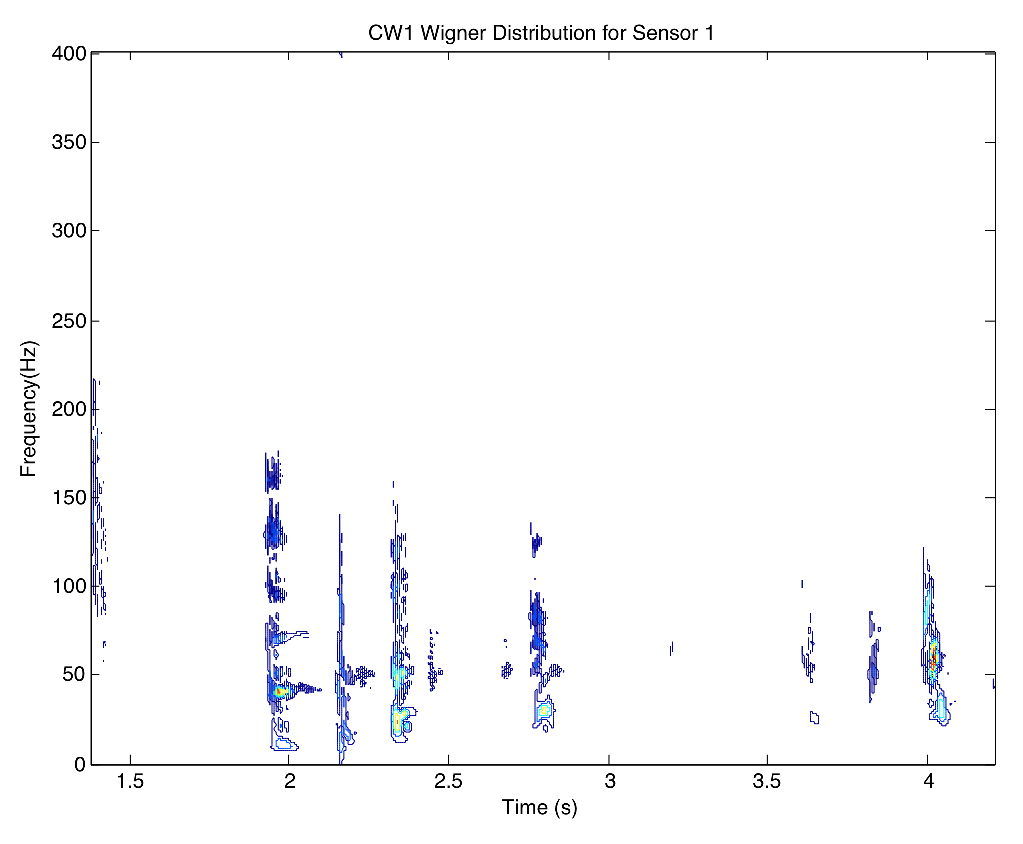
\includegraphics[scale = 0.6]{Images/WD.pdf}
\caption{Example of an WD TFR}
\label{fig:WDTFR}
\end{figure}

\subsubsection{Reduced Interference Distribution}
\label{sec:RID}
The Reduced Interference Distribution (RID) with a Hanning kernel was used for analysis in the project. The equation for the RID can be seen below in Equation \eqref{eq:RID} \cite{Auger2005}. The Hanning kernel is one of the common kernels for the RID, and was beneficial in our case, as it is part of Cohen's Class and has the properties of preserving the time marginal, frequency marginal and the energy \cite{Jeong1992}. These features were important when it came to feature extraction, discussed below in section \ref{sec:featex}.
\begin{equation}
\label{eq:RID}
 RIDH_x(t, f) = \infint h(\tau)R_x(t, \tau) e^{-j2\pi f \tau} d\tau
\end{equation}
where
\begin{equation*}
R_x(t,\tau) = \int_{-\frac{|\tau|}{2}}^{\frac{|\tau|}{2}} \frac{g(\nu)}{|\tau|} \bp{1 + \cos\bp{\frac{2\pi\nu}{\tau}}} x\bp{t + \nu + \frac{\tau}{2}}x^*\bp{t + \nu - \frac{\tau}{2}} d\nu
\end{equation*}
where $g(\nu)$ is a time smoothing window and $h(\tau)$ is a frequency smoothing window.

As can be seen in the above equation, the RID is related to the WD; but as the name suggests, the main purpose of the RID is to reduce the amount of interference (i.e. it tries to reduce the amount of cross terms compared to the auto terms in the TFR representation). This is accomplished by applying a smoothing window to the time and frequency axes, as well as filtering the data. It has many of the desirable properties as well as high time and frequency resolution, which makes it a good candidate for analyzing signals via time-frequency signal representation \cite{Jeong1992}. Figure \ref{fig:TFRRID} below depicts an example of the RID performed on the data gathered.

\begin{figure}[H]
\centering
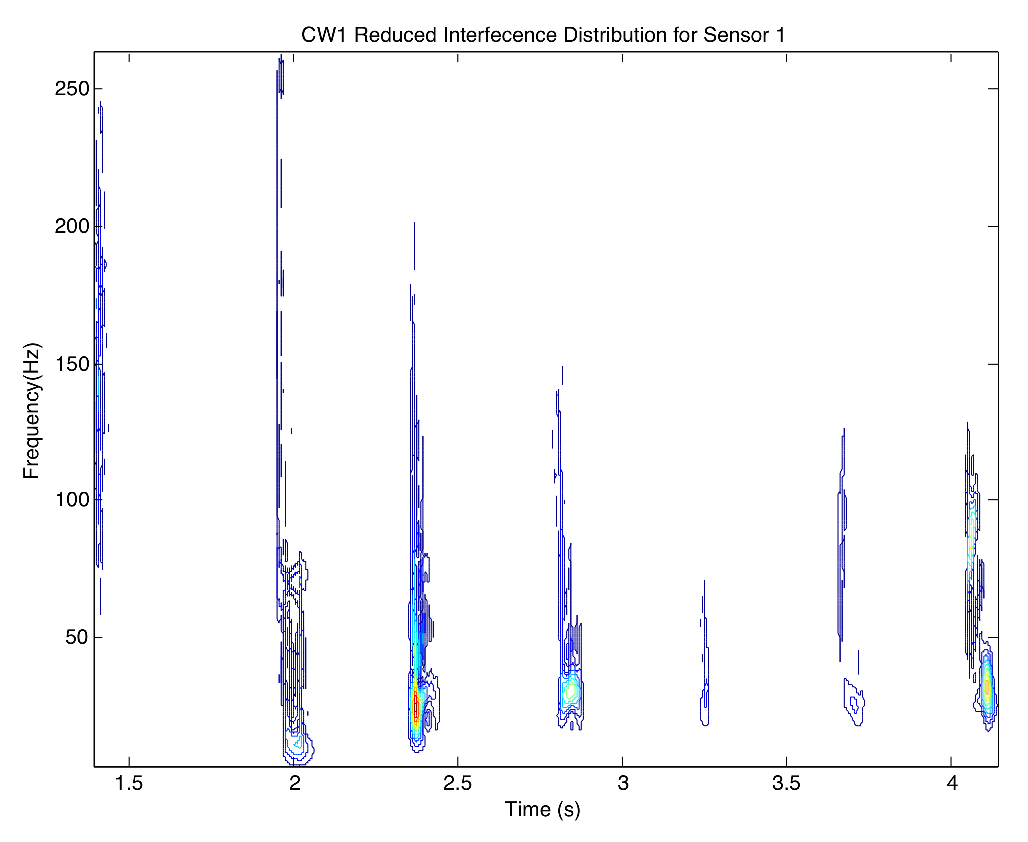
\includegraphics[scale = 0.6]{Images/RID.pdf}
\caption{Example of an RID TFR}
\label{fig:TFRRID}
\end{figure}

\subsection{Feature Extraction}
\label{sec:featex}
Feature extraction begins when we transform our time-domain data into the time-frequency domain.  Each different TFR type may neglect or amplify certain features within the data.  However, we cannot proceed directly to classification, due to the high dimensionality of the TFR. High dimensional data is a challenge often faced when attempting to classify types of data. We explored two possible methods by which we can remove the redundant TFR data and extract only useful features.  The first method is Principal Component Analysis (PCA) and the other is Linear Discriminant Analysis (LDA).

PCA is a statistical method which uses orthogonal projections to represent high dimensional data in a lower-dimensional form. The first principal component is in the direction along which there is the greatest data variance. The next component will project along a direction orthogonal to the first which has the next largest variance. The first principal component accounts for the largest percentage of data variance, with smaller percentages accounted for by each successive component. Depending on the desired final dimension and accuracy of representation, the user may select a limited number of these principal components to represent their data. While PCA is an effective dimensionality reduction technique, it only extracts features that describe a pattern. PCA does not take into account differences in classes, so it cannot effectively extract the features which distinguish between two different patterns.  Our goal is to classify data based on their differences, so PCA will not extract the most useful features. 

In contrast to PCA, LDA specifically extracts features which characterize  the differences between two classes of data. The goal is to reduce dimensionality while preserving class discriminatory information. LDA accomplishes this task by projecting the data along a line (or lower dimension) which maximizes between-class scatter while minimizing within-class scatter. Once the data has been sufficiently separated, it may either be classified using the LDA or sent to a different type of classifier.   

\begin{figure}[H]
   \centering
   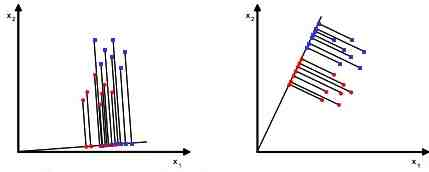
\includegraphics[scale = 0.6]{Images/Bad LDA.jpg} % requires the graphicx package
   \caption{Examples of a Bad Projection Vector (left) and a Good Projection Vector (right) \cite{GutierrezPP}}
   \label{fig:ProjVect}
\end{figure}

We chose to use LDA as our means of dimension reduction, because our focus is on discriminating between various classes and LDA outperforms PCA when extracting class-specific features. The figure below demonstrates the differences between PCA and LDA in terms of class discrimination.

\begin{figure}[H]
   \centering
   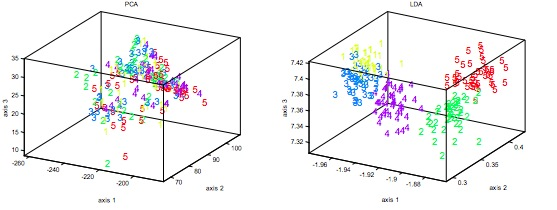
\includegraphics[scale = 0.6]{Images/PCAvLDA.jpeg} % requires the graphicx package
   \caption{3D Scatter Plots for Class Discrimination for PCA (left) and LDA (right)\cite{GutierrezPP}}
   \label{fig:PCALDA}
\end{figure}

\subsection{Classification}
\label{sec:classify}
In order to make implementation of classification in \Matlab \ as practical and accurate as possible, we used a branching tree of binary decisions. These binary classifications allow us to focus on a limited set of features for each branch.

\begin{figure}[H]
   \centering
   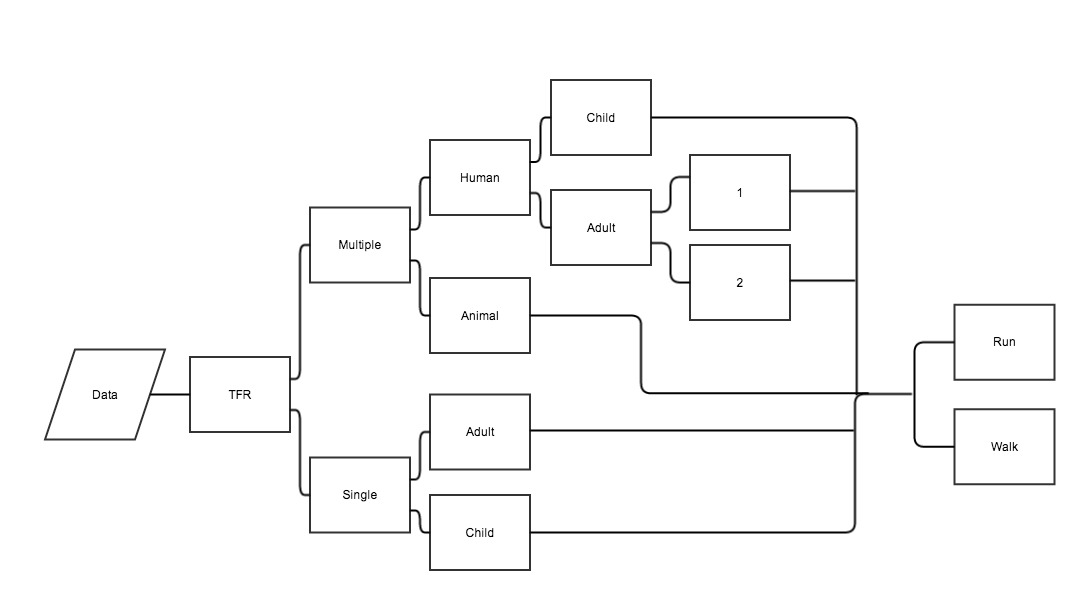
\includegraphics[scale = 0.4]{Images/Decision Tree.jpg} % requires the graphicx package
   \caption{Depiction of Binary Decisions for Classification}
   \label{fig:BinTree}
\end{figure}

At each junction, we tested two types of supervised classifiers, a Support Vector Machine (SVM) and a Linear Discriminant Analysis (LDA).

The simplest classifier is an extension of the LDA dimension reduction. The LDA classifier draws a boundary between two separate classes.  The boundary can be formed with a variety of functions.  We tested LDA using a linear classifier and a quadratic classifier.  Due to the complexity of real data and imperfect separation of classes, a linear boundary is often inadequate in classification. The quadratic classifier performs much better than the linear. 

The SVM creates support vectors from the data points closest to the boundary between two classes.  These points are the most difficult to classify accurately.  Based on these support vectors, the SVM finds an optimal boundary for separating the classes. The shape of the drawn boundary also depends upon the kernel of the SVM. The radial-basis function is one the most commonly used kernel.  It effectively creates a bump around each support vector along the boundary. 
While a capable classifier is important, the most critical step in classification is actually feature extraction.  If the best features are extracted, the classes may be sufficiently separated that even a linear classifier can easily distinguish them.  Whereas even the best classifier will not allow two poorly separated classes to be identified.

%%%%%%%%%%%%%%%%%%%%%%%%%%%%%%%%%%%%%%%%%%%%%%%%%%%%%%
%\vspace{-10pt}
\section{Results}
\label{sec:results}
Prior to performing the classification, the matrix was reduced in order to feasibly process the data. This was accomplished by looking at a specific region in relation to the maximum achieved by the center point.  Each column of this matrix was stacked to form a row feature vector.  The Fisher LDA was then used to reduce the dimension of each TFR vector. The reduced features were then classified using SVM, linear discriminant, and quadratic discriminant.
\subsection{Multiple v. Single}

\begin{table}[H] 
\caption{Results for Multiple (M) v. Single (S)}
\begin{center}
\begin{tabulary}{\textwidth}{ C || C | C | C | C | C | C| }
 & RID & PWD & WD & AF & Spectrogram & MPD \\
 \hline
 \hline
 \multirow{2}{*}{SVM} & M: 48.75\% & M: 53.75\% & M: 67.5\% & \multirow{2}{*}{N/A} & \multirow{2}{*}{N/A} & M: 76.7\% \\
 & S: 28.75\% & S: 26.25\% & S: 20\% & & & S: 75\%\\
 \hline
\multirow{2}{*}{Linear} & M: 40\% & M: 35\% & M: 32.5\% & M:  12.5\% & M: 56.25\% & M: 20\%\\
& S: 35\% & S: 35\% & S: 31.25\% & S: 81.25\% & S: 81.25\%  y& S: 80\%\\
 \hline
\multirow{2}{*}{Quadratic} & M: 45\% & M: 45\% & M: 43.75\% & M: 100\% & M: 92.5\%  & M: 12.5\%\\
 & S: 36.25\% & S: 32.5\% & S: 42.5\% & S: 2.5\% & S: 16.5\%  & S: 90\%\\
 \hline
\end{tabulary}
\end{center}
\end{table}

We were unable to distinguish multiple people from a single person. However, some of the issue from this may have come from multiple people walking abreast in lockstep. Thus, the sensors may not have been able to determine a difference between a group of people and a single person. Figure \ref{fig:MultSigLDA} shows an example of poor separation of the features, which led to poor results.

\begin{figure}[H]
\centering
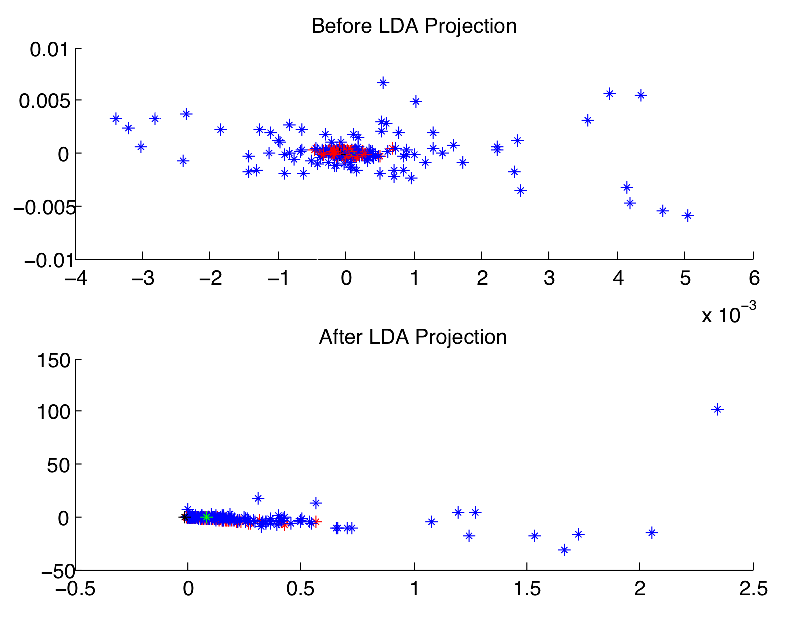
\includegraphics[scale = 0.6]{Images/MultSingle_LDA_plot.pdf}
\caption{Example of Poor Separation between Features}
\label{fig:MultSigLDA}
\end{figure}

\subsection{Adult v. Child}

\begin{table}[H] 
\caption{Results for Adult (A) v. Child (C)}
\begin{center}
\begin{tabulary}{\textwidth}{ C || C | C | C | C | C | C| }
 & RID & PWD & WD & AF & Spectrogram & MPD \\
 \hline
 \hline
 \multirow{2}{*}{SVM} & A: 92.5\% & A: 92.5\% & A: 90\% & \multirow{2}{*}{N/A} & \multirow{2}{*}{N/A} & A: 95.8\% \\
 & C: 67.5\% & C: 65\% & C: 75\% & & & C: 70\%\\
 \hline
 \multirow{2}{*}{Linear} & A: 90\% & A: 82.5\% & A: 85\% & A: 65\% & A: 82.5\% & A: 20\% \\
 & C: 77.5\% & C: 77.5\% & C: 80\% & C: 17.5\% & C: 42.5\% & C: 82.5\%\\
 \hline
 \multirow{2}{*}{Quadratic} & A: 97.5\% & A: 95\% & A: 95\% & A: 0\% & A: 27.5\% & A: 15\% \\
 & C: 80\% & C: 82.5\% & C: 85\% & C: 97.5\% & C: 75\% & C: 87.5\%\\
 \hline
 \end{tabulary}
 \end{center}
 \end{table}
 
We were able to successfully distinguish between the footsteps of an adult and those of child. This is most likely due to the difference in gaits between the adult and child from differences such as height. Since this comparison is between a single adult and a single child, the lockstep problem wouldn't be an issue, and it would showcase the natural gait of both parties, allowing for the classification to take place. Figures \ref{fig:ACLDA} and \ref{fig:ACSVM} show the LDA feature separation, and the resulting classification by the SVM respectively.

\begin{figure}[H]
\centering
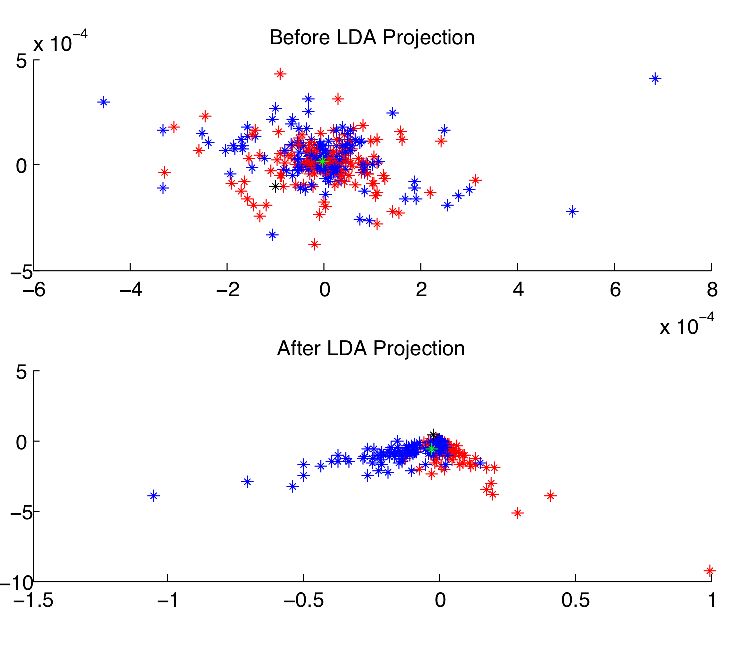
\includegraphics[scale = 0.6]{Images/AdultChild_LDA_goodplot.pdf}
\caption{Example of Good Separation between Features}
\label{fig:ACLDA}
\end{figure}

\begin{figure}[H]
\centering
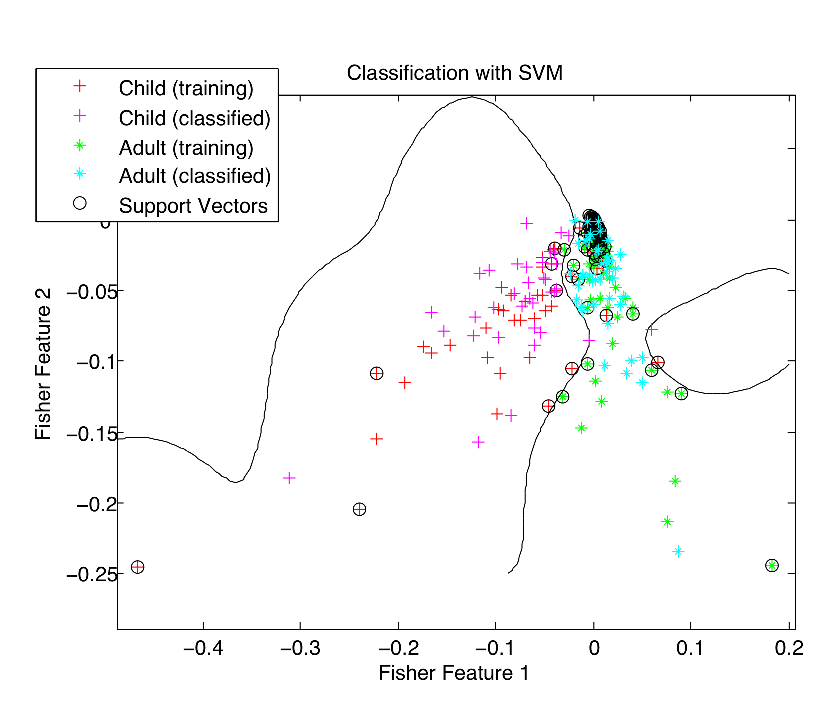
\includegraphics[scale = 0.6]{Images/AdultChild_SVM.pdf}
\caption{SVM Classification based on Fischer LDA Feature Extraction}
\label{fig:ACSVM}
\end{figure}

\subsection{Adult Run v. Adult Walk}
\label{sec:ARAW}
\begin{table}[H] 
\caption{Results for Adult Run (R) v. Adult Walk (W)}
\begin{center}
\begin{tabulary}{\textwidth}{ C || C | C | C | C | C | C| }
 & RID & PWD & WD & AF & Spectrogram & MPD \\
 \hline
 \hline
 \multirow{2}{*}{SVM} & R: 100\% & R: 100\% & R: 100\% & \multirow{2}{*}{N/A} & \multirow{2}{*}{N/A} & R: 96.7\%\\
 & W: 85\% & W: 90\% & W: 90\% & & & W: 100\%\\
 \hline
 \multirow{2}{*}{Linear} & R: 100\% & R: 100\% & R: 100\% & R: 25\% & R: 100\% & R: 100\%\\
 & W: 80\% & W: 80\% & W: 80\% & W: 60\% & W: 60\% & W: 95\%\\
 \hline
 \multirow{2}{*}{Quadratic} & R: 100\% & R: 100\% & R: 100\% & R: 95\% & R: 100\% & R: 100\%\\
 & W: 100\% & W: 100\% & W: 100\% & W: 10\% & W: 5\% & W: 95\%\\
 \hline
 \end{tabulary}
 \end{center}
 \end{table}
 
Distinguishing between running and walking within the adult category was relatively simple. When running, the TFR is characterized by two pronounced footsteps and the frequency of each footstep is high.  In the walking TFR, we typically saw only one footstep at a noticeably lower frequency. %Figure \ref{fig:ARAWSVM} shows the classification bounds from the SVM.

%\begin{figure}[H]
%\centering
%\label{fig:ARAWSVM}
%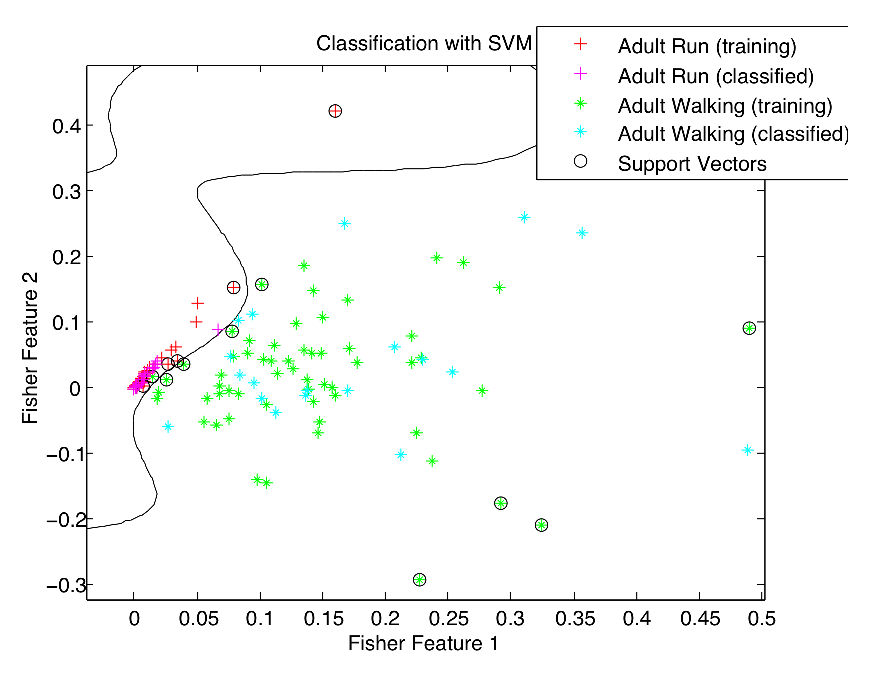
\includegraphics[scale = 0.6]{Images/AdultRunWalk_SVM.pdf}
%\caption{SVM Classification based on Fischer LDA Feature Extraction}
%\end{figure}

\subsection{Child Run v. Child Walk}

\begin{table}[H] 
\caption{Results for Child Run (R) v. Child Walk (W)}
\begin{center}
\begin{tabulary}{\textwidth}{ C || C | C | C | C | C | C| }
 & RID & PWD & WD & AF & Spectrogram & MPD \\
 \hline
 \hline
 \multirow{2}{*}{SVM} & R: 85\% & R: 85\% & R: 85\% & \multirow{2}{*}{N/A} & \multirow{2}{*}{N/A} & R: 83.3\% \\
 & W: 85\% & W: 80\% & W: 85\% & & & W: 85\%\\
 \hline
 \multirow{2}{*}{Linear} & R: 95\% & R: 95\% & R: 95\% & R: 25\% & R: 95\% & R: 80\%\\
 & W: 55\% & W: 50\% & W: 50\% & W: 90\% & W: 50\% & W: 20\%\\
 \hline
 \multirow{2}{*}{Quadratic} & R: 95\% & R: 95\% & R: 95\% & R: 100\% & R: 100\% & R: 90\%\\
 & W: 85\% & W: 85\% & W: 90\% & W: 0\% & W: 0\% & W: 15\%\\
 \hline
 \end{tabulary}
 \end{center}
 \end{table}

We successfully employed the methodology used in distinguishing adult run and walk to classify child run vs. child walking. The reasons for success are similar to those of the adult running and walking discussed above in Section \ref{sec:ARAW}. %Figure \ref{fig:CWCRSVM} shows the classification boundaries from the SVM.

%\begin{figure}[H]
%\centering
%\label{fig:CRCWSVM}
%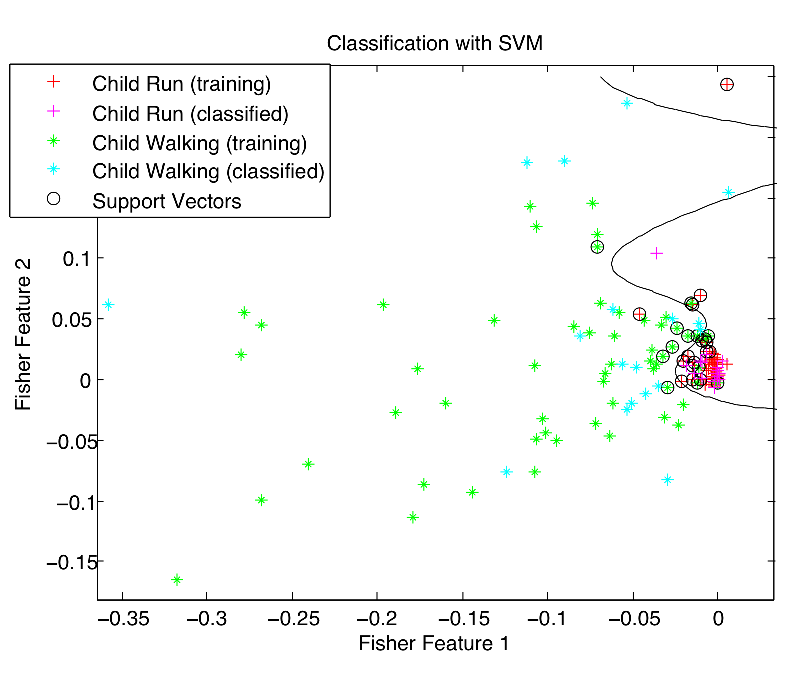
\includegraphics[scale = 0.6]{Images/ChildRunWalk_SVM.pdf}
%\caption{SVM Classification based on Fischer LDA Feature Extraction}
%\end{figure}

%\begin{figure}[H]
%\centering
%\label{fig:ARAWSVM}
%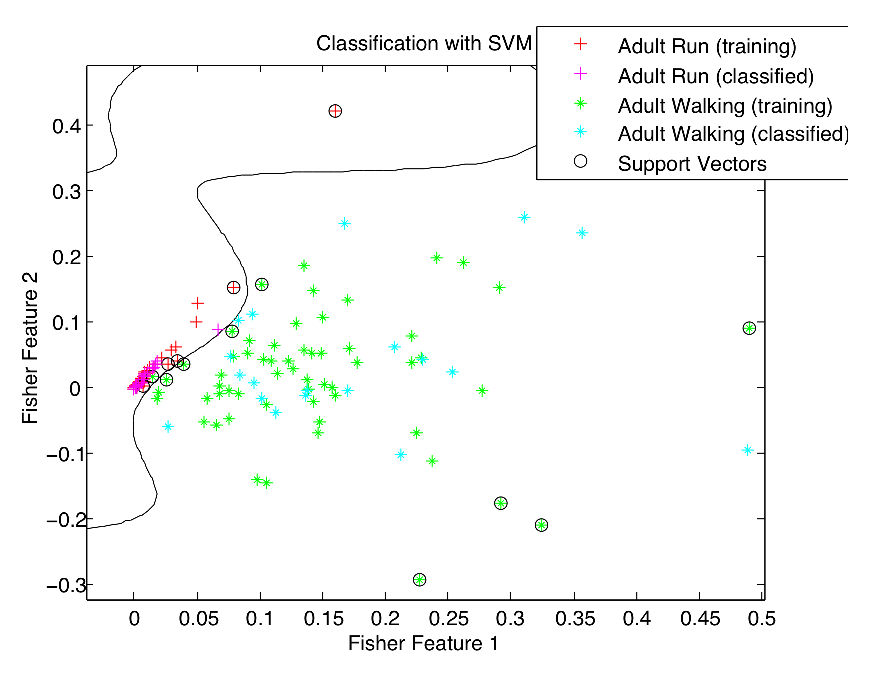
\includegraphics[scale = 0.6]{Images/AdultRunWalk_SVM.pdf}
%\caption{SVM Classification based on Fischer LDA Feature Extraction}
%\end{figure}

\subsection{Adult v. Adult with Dog}

\begin{table}[H] 
\caption{Results for Two Adults (A) v. Adult and Dog (D)}
\begin{center}
\begin{tabulary}{\textwidth}{ C || C | C | C | C | C | C| }
 & RID & PWD & WD & AF & Spectrogram & MPD \\
 \hline
 \hline
 \multirow{2}{*}{SVM} & A: 47.5\% & A: 82.5\% & A: 85\% & \multirow{2}{*}{N/A} & \multirow{2}{*}{N/A} & \multirow{2}{*}{N/A} \\
  & D: 78.33\% & D: 48.3\% & D: 66.6\% & & & \\
 \hline
 \multirow{2}{*}{Linear} & A: 60\% & A: 70\% & A: 60\% & A: 5\% & A: 53.33\% & \multirow{2}{*}{N/A} \\
   & D: 46.6\% & D: 43.4\% & D: 51.6\% & D: 55\% & D: 70\% & \\
 \hline
\multirow{2}{*}{Quadratic} & A: 90\% & A: 92.5\% & A: 92.5\% & A: 100\% & A: 85\% & \multirow{2}{*}{N/A} \\
  & D: 65\% & D: 58.33\% & D: 50\% & D: 5\% & D: 11.67\% & \\
 \hline
 \end{tabulary}
 \end{center}
 \end{table}
 
 When attempting to determine the difference, the results were inconclusive.  We found very little difference between the adult trials and the adult with dog trials.  In \cite{Mehmood2012}, TFR�s were used to distinguish between biped and quadruped motion compared a human and a horse.  Unfortunately, our dog was not large enough to make an impression on the sensors. An additional complication was that the dog had to be lead by an adult past the sensors, resulting in the human vibration patterns overshadowing any useful features that pertained to the dog alone.  Unfortunately, this means that the adult vs. adult and dog trials seem identical. 

\subsection{Adult v. Adult with Child}

\begin{table}[H] 
\caption{Results for Two Adults (A) v. Adult and Child (C)}
\begin{center}
\begin{tabulary}{\textwidth}{ C || C | C | C | C | C | C| }
 & RID & PWD & WD & AF & Spectrogram & MPD \\
 \hline
 \hline
 \multirow{2}{*}{SVM} & A: 52\% & A: 47.5\% & A: 47.5\% & \multirow{2}{*}{N/A} & \multirow{2}{*}{N/A} & A: 90\%\\
 & C: 40\% & C: 50\% & C: 45\% & & & C: 95\%\\
 \hline
\multirow{2}{*}{Linear} & A: 40\% & A: 37.5\% & A: 40\% & A: 50\% & A: 57.5\% & A: 62.5\%\\
& C: 70\% & C: 75\% & C: 85\% & C: 65\% & C: 60\% & C: 80\%\\
 \hline
\multirow{2}{*}{Quadratic} & A: 55\% & A: 52.5\% & A: 50\% & A: 5\% & A: 12.5\% & A: 62.5\%\\
 & C: 60\% & C: 60\% & C: 65\% & C: 90\% & C: 70\% & C: 80\%\\
 \hline
 \end{tabulary}
 \end{center}
 \end{table}
 
 Attempts to determine the difference between two adults walking vs. an adult and a child walking were unsuccessful.  The two adults v. the adult and child comparison suffers from the same problems we saw in the two adults vs. adult with dog. It would appear that the child was too far from the sensors or had too little mass in comparison to the adult. The effect is that the adult footsteps completely masked any child footsteps.  When a child footstep is evident, it is too rare to allow for accurate classification.

\subsection{Two Adults v. Three Adults}
\begin{table}[H] 
\caption{Results for Two Adults (AA) v. Three Adults (AAA)}
\begin{center}
\begin{tabulary}{\textwidth}{ C || C | C | C | C | C | C| }
 & RID & PWD & WD & AF & Spectrogram & MPD \\
 \hline
 \hline
 \multirow{2}{*}{SVM} & AA: 70\% & AA: 80\% & AA: 80\% & \multirow{2}{*}{N/A} & \multirow{2}{*}{N/A} & AA: 78.3\%\\
 & AAA: 65\% & AAA 50\%: & AAA: 65\% & & & AAA: 95\%\\
 \hline
\multirow{2}{*}{Linear} & AA: 75\% & AA: 70\% & AA: 85\% & AA: 30\% & AA: 60\% & AA: 80\%\\
 & AAA: 80\% & AAA: 90\% & AAA: 85\% & AAA: 10\% & AAA: 60\% & AAA: 65\%\\
 \hline
\multirow{2}{*}{Quadratic} & AA: 85\% & AA: 85\% & AA: 90\% & AA: 5\% & AA: 10\% & AA: 80\%\\
 & AAA: 70\% & AAA: 85\% & AAA: 85\% & AAA: 90\% & AAA: 95\% & AAA: 65\%\\
 \hline
 \end{tabulary}
 \end{center}
 \end{table}
 
 We successfully classified the difference between two adults and three adults using our extracted features. %The SVM classification boundaries are shown below in Figure \ref{fig:AAAAASVM}
 
%\begin{figure}[H]
%\centering
%\label{fig:AAAAASVM}
%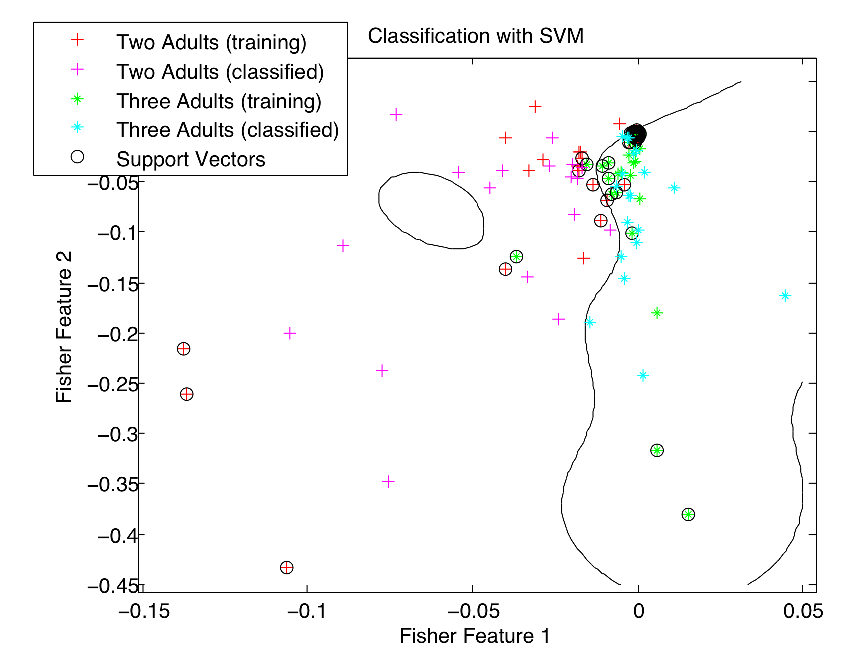
\includegraphics[scale = 0.6]{Images/twoAdultthreeAdult_SVM.pdf}
%\caption{SVM Classification based on Fischer LDA Feature Extraction}
%\end{figure}

%%%%%%%%%%%%%%%%%%%%%%%%%%%%%%%%%%%%%%%%%%%%%%%%%%%%%%
%\vspace{-10pt}
\section{Work Management}
\label{sec:work}
To accomplish the work, everyone in the group had an important role to play. All group members assisted in the gathering of data, acting as test subjects, along with running the data acquisition system. While all members were active in many aspects of the project, the sections below describe the portions of the project each member was the lead on.
\subsection{Kaitlyn Beaudet}
\label{sec:Kaitlyn} 
For the project, Kaitlyn Beaudet was responsible for writing the \Matlab \ code to compile the data acquisition. Additionally, she completed the \Matlab \ code to compute, plot and save the RID, as well as the programming to center the data. Kaitlyn also was responsible for keeping the data organized in \Matlab \ for use in the various sections of code. For the report, Kaitlyn was responsible for writing the the abstract, as well as the introduction, data acquisition, RID and sections of the results. She was also responsible for compiling the final report in \LaTeX \ and organizing the references. 
\subsection{Brett Larsen}
\label{sec:Brett}
In preparation for collecting data, Brett set up both the geophone sensors and the Matlab code for collecting data. This involved mastering the Data Acquisition toolbox as well as determining how to arrange the sensors in the field for data collection. Once the data was in \Matlab, Brett was primarily responsible for updating the code to simultaneously run through and save the TFR generated for each signal by MPD as well as each signal's feature vector. Next, Brett wrote new code to perform MPD using a dictionary of previously recorded signals that saves the type of dictionary elements used to represent the inputted signal and compares this to the actual signal type for classification. Lastly, Brett ran both LDA and SVM on all the TFR's generated by MPD and determined their classification accuracy. For the final report, Brett wrote part of the abstract, the section on matching pursuit, and the conclusion. He also edited the report overall for grammar and accuracy.
\subsection{Lydia Letham}
\label{sec:Lydia}
In the data preprocessing stage, Lydia was in charge of determining how much downsampling was possible and writing \Matlab \ code to implement the downsampling for all data trials.  Lydia wrote the \Matlab \ code to calculate and plot the PWD. Lydia was also responsible for the feature extraction stage.  She determined the distinguishing TFR features for each binary classification decision. I.e., the differences between running and walking, or multiple people vs. single person. Lydia wrote the \Matlab \ code which created a feature vector for each TFR.  Then, she implemented LDA in \Matlab \ to reduce the TFR feature vector to a more manageable size before classification.  Lydia also wrote \Matlab \ code to implement classification using Linear Discriminant, Quadratic Discriminant, and SVM. In the report, Lydia was responsible for writing the WD, feature extraction, and classification sections.  As well as contributing to the writing of the results section.
\subsection{Tianran Liu}
\label{sec:Tianran}
For the project, Tianran Liu was in charge of writing the \Matlab\ code to analyze the signal using spectrogram method. Additionally, she implemented on writing the \Matlab\ code to analyze using ambiguity function, which computes, plots and saves the ambiguity function. In the process of  writing the final report, she was responsible of stating the background information of the entire project. She was also responsible for writing the methods of analysis techniques with spectrogram and ambiguity function.

%\vspace{-10pt}
\section{Conclusions and Future Work}
\label{sec:conclusion}
We were able to compare and contrast the classification results of the WD and the PWD. The PWD TFR plots were cleaner as a result of the smoothing in the frequency direction.  However, perhaps because of the smoothing, the WD generally outperformed the PWD in terms of classification. Similar to the PWD, RID smooths in both time and frequency directions. We noticed that the WD also performed better than RID.  Lastly, MPD performed very well in most classifications.  By providing a TFR free of cross-terms, MPD performed on par  with RID.

Ambiguity and spectrogram feature extraction was not successful.  For both of these methods, our classification results were inconclusive for SVM, and the linear and quadratic classifier results were inaccurate when compared to the results consistently obtained using other TFRs such as RID, WD and PWD. We determined that in the cases of ambiguity and spectrogram, our feature extraction was insufficient to accurately represent and distinguish between various TFRs. 

In addition to certain TFR's being mores successful than others, certain types of classification were more successful than others.  RID, WD, and MPD were able to successfully distinguish between an adult and a child, an adult running and an adult walking, a child running and a child walking, and two and three adults.  In all these cases, we were able to extract some distinctive feature, such as the spacing of the footsteps or overall energy in the signal.

Other cases were not as successful.  Distinguishing between an adult and an adult with dog was inconclusive, and separating data from two adults versus an adult with a child and multiple people versus an individual were unsuccessful.  This child and dog tests likely failed because the strength of the footsteps from the adult drowned out the signals from the lighter child or dog.  One problem with the multiple people versus individual classification was occasionally the group walked in lock step, resulting in the signal appearing to have one set of heavy footsteps. 

In the future, we plan to continue this work by developing other methods of feature extraction and classification, such as the MPD algorithm with a real data dictionary and random projection.  We also plan to manually extract some features such as the time-frequency concentration, or the amount of energy in a box in the time-frequency domain.  For distinguishing a dog versus a human, we plan to try obtain some data without the human walking beside the dog.  And finally, we plan to attempt to use some unsupervised clustering methods to make the classification more adaptive for use in different terrains.

\section{Acknowledgements}
\label{sec:Ack}
The team would like to acknowledge Dr. Narayan Kovvali and Dr. Antonia Papandreou for contributing the starting Matlab code for Matching Pursuit Decomposition.  In addition, the team would like to thank Stavros Papandreou for his help in collecting seismic signals as well as Vipin Vijayan for his Direct LDA toolbox \cite{Vijayan}


%Bibliography
\bibliographystyle{IEEEtran}
\bibliography{proposal_refs.bib}

\end{document}